\section{World Models and Environment Interaction}

\begin{frame}{}
    \LARGE Agentic Models: \textbf{World Models and Environments}

    \vspace{1em}
    \normalsize Can an agent try an action in its head before it tries it in the world?
\end{frame}

\begin{frame}{Three Ways to Choose the Next Action}
    \centering
    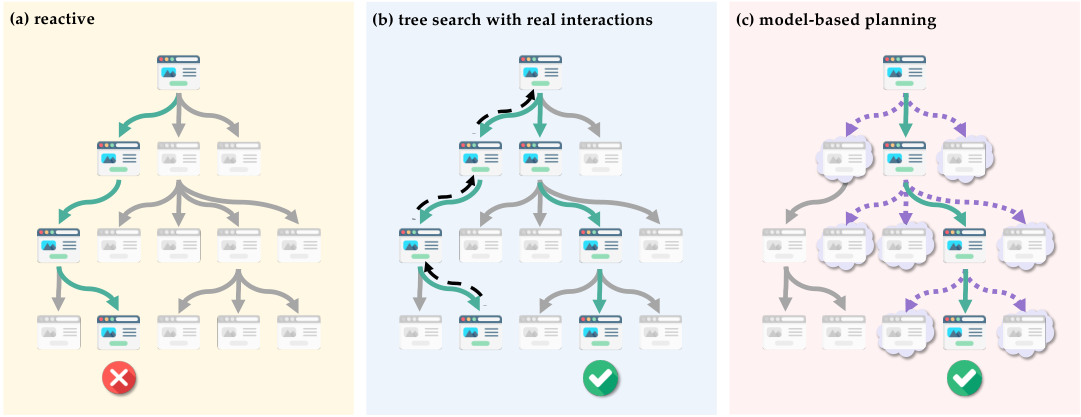
\includegraphics[width=0.9\linewidth,height=0.42\textheight,keepaspectratio]{images/agentic-models-memory/webdreamer_fig1_paradigms.png}
    \begin{itemize}\itemsep0.35em
        \item For LLM agents, a \textbf{world model} predicts state changes \emph{in text}.
        \item Reactive agents are greedy. Real tree search is systematic, but real actions can be \alert{irreversible, unsafe and slow}. So simulate first.
    \end{itemize}
    \src{Figure: Gu et al., ``Is Your LLM Secretly a World Model of the Internet?'' (WebDreamer), \href{https://arxiv.org/abs/2411.06559}{arXiv:2411.06559}, Figure 1. Su, ``On Memory, Reasoning, and Planning of Language Agents,'' Berkeley CS294 (Feb 2025).}
\end{frame}

\begin{frame}{One-Step Lookahead on the Web}
    \begin{columns}[T,onlytextwidth]
        \column{0.5\textwidth}
        \begin{itemize}\itemsep0.45em
            \item \textbf{WebDreamer.} For each candidate action, the LLM imagines the outcome, scores it (1.0 complete, 0.5 on track, 0 wrong), and takes the best:
            \[
                a_t = \arg\max_{a}\ \mathrm{score}\big(\mathrm{sim}(o_t,a)\big)
            \]
            \item \textbf{The best horizon is one step.} At two or three steps, errors accumulate.
            \item \textbf{WMA} predicts only \emph{what changes} between pages, in natural language. It costs \$0.4 per task against \$2.7 for tree search.
        \end{itemize}
        \column{0.48\textwidth}
        \centering
        \small
        \renewcommand{\arraystretch}{1.15}
        \begin{adjustbox}{max width=\linewidth}\begin{tabular}{>{\raggedright\arraybackslash}p{2.5cm}ccc}
            \toprule
            \textbf{Success (\%)} & \textbf{Reactive} & \textbf{Tree} & \textbf{Dreamer} \\
            \midrule
            VisualWebArena & 17.6 & \textbf{26.2} & 23.6 \\
            Online-Mind2Web & 26.0 & n/a & \textbf{37.0} \\
            Mind2Web-Live & 20.2 & n/a & \textbf{25.0} \\
            \midrule
            Seconds per task & 79.8 & 835.7 & 198.9 \\
            \bottomrule
        \end{tabular}\end{adjustbox}

        \vspace{0.4em}
        {\footnotesize Tree search cannot run on live sites: actions there cannot be undone.}
    \end{columns}
    \vspace{0.3em}
    \takeaway{Simulation recovers most of the benefit of search, and it is the \textbf{only} option when actions are irreversible.}
    \src{Gu et al., \href{https://arxiv.org/abs/2411.06559}{arXiv:2411.06559}, Tables 1 and 2 (time is a mean over three sites). Chae et al., ``Web Agents with World Models,'' \href{https://arxiv.org/abs/2410.13232}{arXiv:2410.13232}.}
\end{frame}

\begin{frame}{How Good Are LLM Simulators?}
    \begin{columns}[T,onlytextwidth]
        \column{0.5\textwidth}
        \centering
        \begin{adjustbox}{max width=\linewidth}\begin{tikzpicture}
            \begin{axis}[
                xbar, bar width=9pt, width=7.0cm, height=4.3cm,
                xmin=0, xmax=100, xlabel={next-state prediction accuracy (\%)},
                symbolic y coords={Env-driven,Web pages,Action-driven,Humans},
                ytick=data, y tick label style={font=\scriptsize},
                x label style={font=\scriptsize}, x tick label style={font=\scriptsize},
                nodes near coords, nodes near coords style={font=\scriptsize},
                axis lines*=left, xmajorgrids, grid style={gray!20}, enlarge y limits=0.2]
                \addplot[fill=KAUSTcyan!55, draw=KAUSTcyan!70!black] coordinates {(49.7,Env-driven) (54.75,Web pages) (77.1,Action-driven) (80,Humans)};
            \end{axis}
        \end{tikzpicture}\end{adjustbox}

        {\scriptsize GPT-4 on text-game transitions. Web pages: average over LLMs.}
        \column{0.48\textwidth}
        \begin{itemize}\itemsep0.45em
            \item LLMs predict what \emph{their own action} does. They get only about half right on what the \emph{environment} does next by itself.
            \item \textbf{Do they hold a coherent world model?} A transformer trained on New York taxi routes predicts next turns perfectly, yet its implied street map is incoherent.
            \item With 10\% random detours, its valid-route rate falls to 0.08.
        \end{itemize}
    \end{columns}
    \vspace{0.3em}
    \takeaway{Today's LLM world models are \emph{local, one-step critics}.}
    \src{Wang et al., ``Can Language Models Serve as Text-Based World Simulators?'' \href{https://arxiv.org/abs/2406.06485}{arXiv:2406.06485}. Chae et al., \href{https://arxiv.org/abs/2410.13232}{arXiv:2410.13232}. Vafa et al., ``Evaluating the World Model Implicit in a Generative Model,'' \href{https://arxiv.org/abs/2406.03689}{arXiv:2406.03689}.}
\end{frame}

\begin{frame}{Environment Interaction: Computer Use as the Hard Case}
    \begin{center}
    \small
    \renewcommand{\arraystretch}{1.2}
    \begin{adjustbox}{max width=\linewidth}\begin{tabular}{>{\raggedright\arraybackslash}p{3.3cm}>{\raggedright\arraybackslash}p{4.6cm}>{\raggedright\arraybackslash}p{5.2cm}}
        \toprule
        \textbf{Benchmark} & \textbf{Setup} & \textbf{Result} \\
        \midrule
        OSWorld (Apr 2024) & 369 tasks in real virtual machines & humans 72.36\%, best model 12.24\% \\
        OSWorld-Verified (Jul 2025) & 300+ issues fixed & best agent 60.76\% \\
        \rowcolor{KAUSTcyan!12} OSWorld 2.0 (Jun 2026) & 108 tasks, median 1.6 human hours & Claude Opus 4.8: \textbf{20.6\%} complete, 54.8\% partial \\
        \bottomrule
    \end{tabular}\end{adjustbox}
    \end{center}
    \begin{itemize}\itemsep0.45em
        \item \textbf{What failed in 2024:} over 75\% of analysed failures were inaccurate clicks. A \emph{grounding} problem.
        \item \textbf{What fails in 2026:} losing track of constraints. All models score zero on tasks beyond 163 minutes.
    \end{itemize}
    \src{Xie et al., ``OSWorld,'' \href{https://arxiv.org/abs/2404.07972}{arXiv:2404.07972}. XLANG Lab, ``Introducing OSWorld-Verified'' (Jul 2025). Yuan et al., ``OSWorld 2.0,'' \href{https://arxiv.org/abs/2606.29537}{arXiv:2606.29537}.}
\end{frame}

\begin{frame}{Environments Became Training Infrastructure}
    \begin{columns}[T,onlytextwidth]
        \column{0.36\textwidth}
        \centering
        \begin{adjustbox}{max width=\linewidth}\begin{tikzpicture}[font=\footnotesize, >=Stealth,
            b/.style={draw, rounded corners=2pt, minimum width=3.9cm, minimum height=0.9cm, align=center, text width=3.7cm}]
            \node[b, fill=gray!12] (a) at (0,3.0) {\textbf{Executable state}\\with reset};
            \node[b, fill=darkorange!20] (b) at (0,1.7) {\textbf{Verifier}\\this \emph{is} the reward};
            \node[b, fill=KAUSTcyan!20] (c) at (0,0.4) {\textbf{Task generator}};
            \node[gray, font=\scriptsize] at (0,-0.4) {three parts of an environment};
        \end{tikzpicture}\end{adjustbox}
        \column{0.62\textwidth}
        \begin{itemize}\itemsep0.45em
            \item \textbf{SWE-Gym, R2E-Gym.} Thousands of repository tasks with runnable tests. R2E-Gym generates 8.7K+ of them procedurally from commits.
            \item \textbf{Open environments.} Prime Intellect's hub packages each one as dataset, rubric and interaction loop: 400+ in two months.
            \item \textbf{World modelling as a training objective.} Meta's Code World Model spends about 5T tokens on predicting Python execution traces line by line.
        \end{itemize}
    \end{columns}
    \vspace{0.3em}
    \takeaway{This is the supply side of the open-lab agentic RL recipe: \textbf{the environment is the dataset}.}
    \src{Pan et al., ``SWE-Gym,'' \href{https://arxiv.org/abs/2412.21139}{arXiv:2412.21139}. Jain et al., ``R2E-Gym,'' \href{https://arxiv.org/abs/2504.07164}{arXiv:2504.07164}. Prime Intellect, Environments Hub posts (2025). Meta FAIR CodeGen, ``CWM,'' \href{https://arxiv.org/abs/2510.02387}{arXiv:2510.02387}, and model card.}
\end{frame}

\begin{frame}{Training in Imagination}
    \begin{columns}[T,onlytextwidth]
        \column{0.6\textwidth}
        \begin{itemize}\itemsep0.4em
            \item \textbf{DreamGym.} An LLM \emph{experience model} generates states and rewards in abstract text. With \alert{zero real interactions}, WebShop reaches 63.9, against 65.0 for RL on 80K real transitions (Llama-3.1-8B).
            \item \textbf{DynaWeb.} Mix imagined rollouts with real ones. About 40\% real data is the sweet spot.
            \item \textbf{SIMA 2} (right). A Gemini task setter proposes tasks, a Gemini reward model scores them, and the agent retrains on its successes, including inside Genie 3 generated worlds.
        \end{itemize}
        \column{0.38\textwidth}
        \centering
        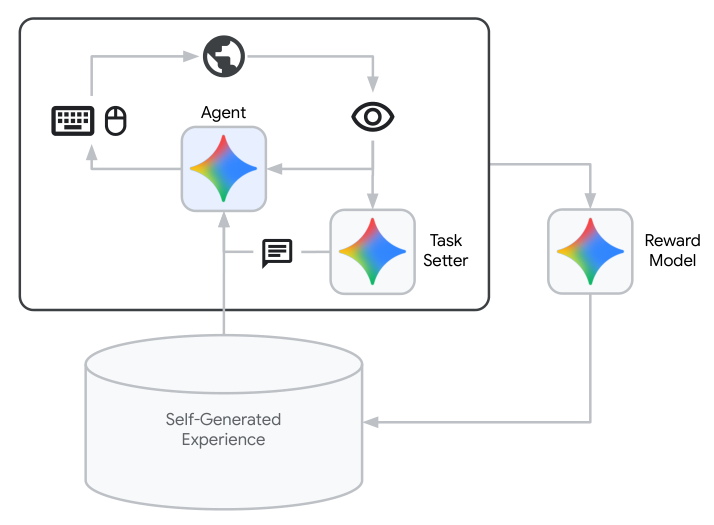
\includegraphics[width=\linewidth,height=0.5\textheight,keepaspectratio]{images/agentic-models-memory/sima2_fig16_self_improvement.png}
    \end{columns}
    \vspace{0.2em}
    \caveat{Simulators are \textbf{sycophantic}: WebWorld reports ``overly optimistic outcomes that cater to the agent's action''.}
    \src{Chen et al., ``DreamGym,'' \href{https://arxiv.org/abs/2511.03773}{arXiv:2511.03773}. Ding et al., ``DynaWeb,'' \href{https://arxiv.org/abs/2601.22149}{arXiv:2601.22149}. Xiao et al., ``WebWorld,'' \href{https://arxiv.org/abs/2602.14721}{arXiv:2602.14721}. Figure: Google DeepMind SIMA team, ``SIMA 2,'' \href{https://arxiv.org/abs/2512.04797}{arXiv:2512.04797}, Figure 16.}
\end{frame}

\begin{frame}{World Models: What to Remember}
    \begin{center}
    \small
    \renewcommand{\arraystretch}{1.2}
    \begin{adjustbox}{max width=\linewidth}\begin{tabular}{>{\raggedright\arraybackslash}p{5.4cm}>{\raggedright\arraybackslash}p{7.4cm}}
        \toprule
        \textbf{Situation} & \textbf{Reasonable choice (our synthesis)} \\
        \midrule
        Environment is cheap to reset, policy is strong & stay reactive and model-free \\
        Actions are irreversible or slow & one-step lookahead with an LLM world model \\
        No RL infrastructure, or real data is scarce & synthetic experience, always mixed with real data \\
        \bottomrule
    \end{tabular}\end{adjustbox}
    \end{center}
    \begin{itemize}\itemsep0.5em
        \item LLM world models work as \textbf{local critics}. They are weak on environment-driven change and on long rollouts.
        \item The same trained model now serves as inference-time critic, synthetic-data generator and environment substitute.
    \end{itemize}
    \vspace{0.2em}
    \takeaway{\textbf{Next.} Every claim so far rested on a benchmark number. How far can those be trusted?}
    
\end{frame}
